% =====================================================================================
% Figure 1 -- Unified RI -> MaRI -> CRoMa conceptual schematic.
%
% One shared neighbourhood, read three ways:
%   A) RI    -- count typed neighbours inside a fixed-k window (distance-blind).
%   B) MaRI  -- same window, weight each typed neighbour by distance (thick edge = close).
%   C) CRoMa -- drop the window; compare distance to the nearest SO vs nearest OS (k-free).
%
% The point constellation is IDENTICAL across all three panels (macro \neighbourhood),
% so the reader sees the same neighbourhood re-read. Colours / node styles / knncircle /
% panelframe are reused verbatim from figures/ri_mari.tex; the Model-A layout and the
% panel-B edge weights are the same Model A used there (RI=0.60, MaRI=0.43), extended
% here with the CRoMa reading on the same points (nearest OS ~3x closer than nearest SO
% => CRoMa=-0.52). The reading flips across balance as margin-awareness increases:
% RI 0.60 (>0.5, biology by count) -> MaRI 0.43 (<0.5, confounder once weighted)
% -> CRoMa -0.52 (<0, strongly confounder-dominant, no k).
%
% Compile: pdflatex concept_metrics.tex  ->  concept_metrics.pdf
% Included by sections (methods.tex) via \includegraphics{figures/concept_metrics.pdf}.
% =====================================================================================
\documentclass[tikz,border=5pt]{standalone}
\usepackage{tikz}
\usetikzlibrary{shapes.geometric,arrows.meta}

% ---- shared neighbourhood: identical point constellation in every panel (anchor at (0,0)) ----
\newcommand{\neighbourhood}{%
  % SO -- cross-confounder biological matches (favourable); three inside the window, one outside
  \node[sopoint] at (-0.70,0.35) {};
  \node[sopoint] at (0.75,0.20) {};
  \node[sopoint] at (0.15,-0.80) {};
  \node[sopoint] at (1.18,0.22) {};
  % OS -- same-confounder distractors; the two closest to the anchor sit inside the window
  \node[ospoint] at (0.20,0.12) {};
  \node[ospoint] at (-0.18,-0.18) {};
  \node[ospoint] at (-1.18,-0.32) {};
  % SS / OO -- uninformative context (never scored)
  \node[sspoint] at (-0.58,0.70) {};
  \node[sspoint] at (-0.15,0.25) {};
  \node[oopoint] at (0.62,-0.40) {};
  \node[oopoint] at (0.98,0.95) {};
}

\begin{document}
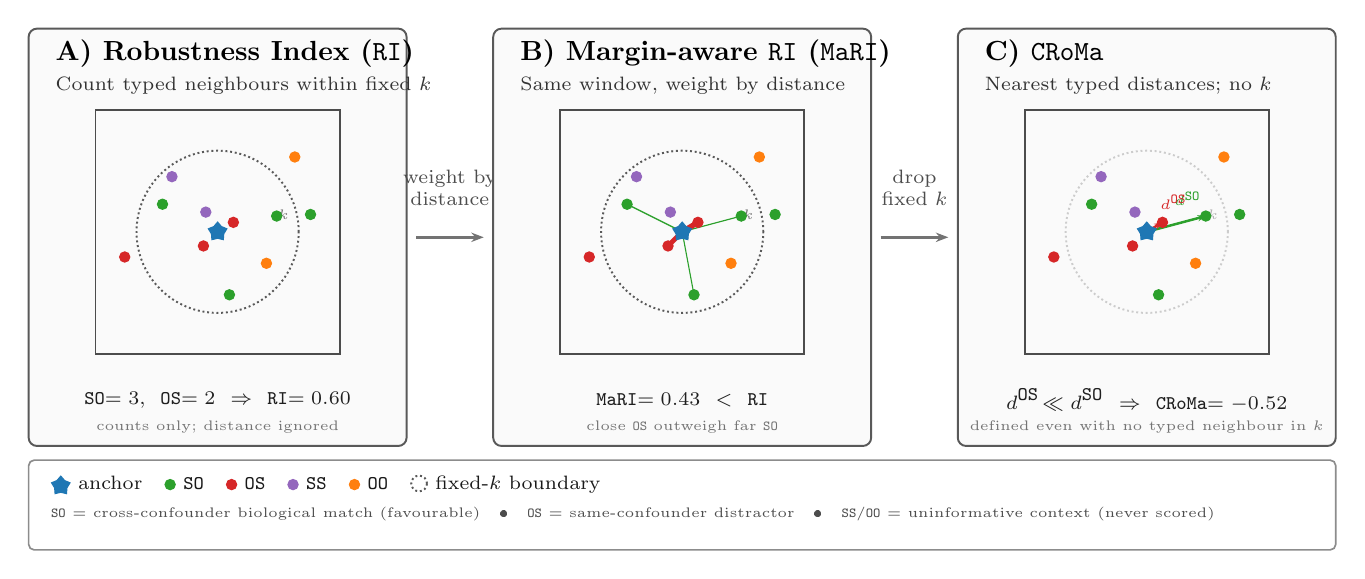
\begin{tikzpicture}[font=\small]
  \definecolor{anchorblue}{RGB}{31,119,180}
  \definecolor{sscol}{RGB}{148,103,189}
  \definecolor{oocol}{RGB}{255,127,14}
  \definecolor{socol}{RGB}{44,160,44}
  \definecolor{oscol}{RGB}{214,39,40}

  \tikzset{
    anchorpt/.style={star,star points=5,fill=anchorblue,draw=anchorblue,minimum size=7pt,inner sep=0pt},
    sspoint/.style={circle,draw=sscol,fill=sscol,minimum size=3.7pt,inner sep=0pt},
    oopoint/.style={circle,draw=oocol,fill=oocol,minimum size=3.7pt,inner sep=0pt},
    sopoint/.style={circle,draw=socol,fill=socol,minimum size=3.7pt,inner sep=0pt},
    ospoint/.style={circle,draw=oscol,fill=oscol,minimum size=3.7pt,inner sep=0pt},
    knncircle/.style={densely dotted,draw=black!65,line width=0.7pt},
    ghostcircle/.style={densely dotted,draw=black!20,line width=0.7pt},
    repspace/.style={draw=black!70,line width=0.65pt},
    panelframe/.style={rounded corners=3pt,draw=black!65,fill=black!2,line width=0.7pt},
    distarrow/.style={-{Stealth[length=3pt]},line width=0.9pt},
    stepflow/.style={-{Stealth[length=4.5pt]},line width=1.2pt,draw=black!55}
  }

  % ============================ Panel A: RI (count) ============================
  \begin{scope}[shift={(0,0)}]
    \draw[panelframe] (0,0) rectangle (4.8,5.3);
    \node[anchor=west,font=\bfseries] at (0.22,4.98) {A) Robustness Index (\texttt{RI})};
    \node[anchor=west,font=\scriptsize,text=black!80] at (0.22,4.58) {Count typed neighbours within fixed $k$};

    \begin{scope}[shift={(2.40,2.72)}]
      \draw[repspace] (-1.55,-1.55) rectangle (1.55,1.55);
      \draw[knncircle] (0,0) circle (1.03);
      \node[anchor=south east,font=\tiny,text=black!55] at (1.03,0.03) {$k$};
      \neighbourhood
      \node[anchorpt] at (0,0) {};
    \end{scope}

    \node[font=\scriptsize,text=black!88] at (2.40,0.58)
      {\texttt{SO}$=3$,\ \ \texttt{OS}$=2$\ \ $\Rightarrow$\ \ \texttt{RI}$=0.60$};
    \node[font=\tiny,text=black!55] at (2.40,0.24) {counts only; distance ignored};
  \end{scope}

  % A -> B step
  \draw[stepflow] (4.92,2.65) -- (5.78,2.65);
  \node[font=\scriptsize,text=black!70,align=center] at (5.35,3.28) {weight by\\distance};

  % ============================ Panel B: MaRI (distance-weighted) ============================
  \begin{scope}[shift={(5.90,0)}]
    \draw[panelframe] (0,0) rectangle (4.8,5.3);
    \node[anchor=west,font=\bfseries] at (0.22,4.98) {B) Margin-aware \texttt{RI} (\texttt{MaRI})};
    \node[anchor=west,font=\scriptsize,text=black!80] at (0.22,4.58) {Same window, weight by distance};

    \begin{scope}[shift={(2.40,2.72)}]
      \draw[repspace] (-1.55,-1.55) rectangle (1.55,1.55);
      \draw[knncircle] (0,0) circle (1.03);
      \node[anchor=south east,font=\tiny,text=black!55] at (1.03,0.03) {$k$};

      % weighted typed edges (thick = close). Far SO -> thin; close OS -> thick.
      \draw[socol,line width=0.45pt] (0,0) -- (-0.70,0.35);
      \draw[socol,line width=0.42pt] (0,0) -- (0.75,0.20);
      \draw[socol,line width=0.40pt] (0,0) -- (0.15,-0.80);
      \draw[oscol,line width=1.95pt] (0,0) -- (0.20,0.12);
      \draw[oscol,line width=1.70pt] (0,0) -- (-0.18,-0.18);

      \neighbourhood
      \node[anchorpt] at (0,0) {};
    \end{scope}

    \node[font=\scriptsize,text=black!88] at (2.40,0.58)
      {\texttt{MaRI}$=0.43$\ \ $<$\ \ \texttt{RI}};
    \node[font=\tiny,text=black!55] at (2.40,0.24) {close \texttt{OS} outweigh far \texttt{SO}};
  \end{scope}

  % B -> C step
  \draw[stepflow] (10.82,2.65) -- (11.68,2.65);
  \node[font=\scriptsize,text=black!70,align=center] at (11.25,3.28) {drop\\fixed $k$};

  % ============================ Panel C: CRoMa (k-free margin) ============================
  \begin{scope}[shift={(11.80,0)}]
    \draw[panelframe] (0,0) rectangle (4.8,5.3);
    \node[anchor=west,font=\bfseries] at (0.22,4.98) {C) \texttt{CRoMa}};
    \node[anchor=west,font=\scriptsize,text=black!80] at (0.22,4.58) {Nearest typed distances; no $k$};

    \begin{scope}[shift={(2.40,2.72)}]
      \draw[repspace] (-1.55,-1.55) rectangle (1.55,1.55);
      % the window that RI/MaRI needed is gone -- shown only as a faded, inert ghost
      \draw[ghostcircle] (0,0) circle (1.03);
      \node[anchor=south east,font=\tiny,text=black!30] at (1.03,0.03) {$k$};

      % distance to nearest SO (far) and nearest OS (close), from the same constellation
      \draw[distarrow,socol] (0,0) -- (0.75,0.20);
      \node[font=\tiny,text=socol] at (0.52,0.42) {$d^{\texttt{SO}}$};
      \draw[distarrow,oscol] (0,0) -- (0.20,0.12);
      \node[anchor=south west,font=\tiny,text=oscol] at (0.05,0.16) {$d^{\texttt{OS}}$};

      \neighbourhood
      \node[anchorpt] at (0,0) {};
    \end{scope}

    \node[font=\scriptsize,text=black!88] at (2.40,0.58)
      {$d^{\texttt{OS}}\!\ll d^{\texttt{SO}}$\ \ $\Rightarrow$\ \ \texttt{CRoMa}$=-0.52$};
    \node[font=\tiny,text=black!55] at (2.40,0.24) {defined even with no typed neighbour in $k$};
  \end{scope}

  % ============================ shared legend (two rows: symbols, then SO/OS gloss) ============================
  \draw[draw=black!45,fill=white,rounded corners=2pt,line width=0.6pt] (0,-1.32) rectangle (16.6,-0.18);
  \node[anchor=north west,font=\scriptsize,align=left,text=black!90] at (0.16,-0.24)
    {\raisebox{0.55ex}{\tikz[baseline=-0.55ex]\node[anchorpt]{};} anchor\quad
     \raisebox{0.55ex}{\tikz[baseline=-0.55ex]\node[sopoint]{};} \texttt{SO}\quad
     \raisebox{0.55ex}{\tikz[baseline=-0.55ex]\node[ospoint]{};} \texttt{OS}\quad
     \raisebox{0.55ex}{\tikz[baseline=-0.55ex]\node[sspoint]{};} \texttt{SS}\quad
     \raisebox{0.55ex}{\tikz[baseline=-0.55ex]\node[oopoint]{};} \texttt{OO}\quad
     \raisebox{0.2ex}{\tikz[baseline=-0.55ex]\draw[knncircle] (0,0) circle (0.10);} fixed-$k$ boundary\\[2pt]
     \tiny\textcolor{black!70}{\texttt{SO} $=$ cross-confounder biological match (favourable)\quad\textbullet\quad
       \texttt{OS} $=$ same-confounder distractor\quad\textbullet\quad
       \texttt{SS}/\texttt{OO} $=$ uninformative context (never scored)}};
\end{tikzpicture}
\end{document}
